\documentclass{beamer}
% Some basic packagesLLuu
\usepackage[utf8]{inputenc}
\usepackage{spverbatim}
\usepackage{textcomp}
\usepackage{pgfplots}
\usepackage{url}
\usepackage{graphicx}
\usepackage{float}
\usepackage{algorithm2e}
\usepackage{enumitem}
\usepackage{standalone}
\usepackage{tcolorbox}
\usepackage{wrapfig}
% \usepackage{svg}
% \usepackage{svg-inkscape} 

\graphicspath{{./figures}}

%color settings
\usepackage{xcolor}
\definecolor{gruvbgdark}{HTML}{1d2021}
\definecolor{gruvtextdark}{HTML}{ebdbb2}
\definecolor{gruvbglight}{HTML}{f9f5d7}
\definecolor{gruvtextlight}{HTML}{3c3836}
\definecolor{NavyBlue}{HTML}{266bbd}
\definecolor{RawSienna}{HTML}{94330e}
\definecolor{ForestGreen}{HTML}{149b52}
% \pagecolor{gruvbgdark}
% \color{gruvtextdark}

% Hide page number when page is empty
\usepackage{emptypage}
\usepackage{subcaption}
\usepackage{multicol}

% Math stuff
\usepackage{amsmath, amsfonts, mathtools, amsthm, amssymb}
% Fancy script capitals
\usepackage{mathrsfs}
\usepackage{cancel}

% Bold math
\usepackage{bm}

%Algorithm setup
\RestyleAlgo{algoruled}
% Some shortcuts
\newcommand\N{\ensuremath{\mathbb{N}}}
\newcommand\R{\ensuremath{\mathbb{R}}}
\newcommand\Z{\ensuremath{\mathbb{Z}}}
\renewcommand\O{\ensuremath{\emptyset}}
\newcommand\Q{\ensuremath{\mathbb{Q}}}
\newcommand\C{\ensuremath{\mathbb{C}}}
\newcommand\B{\ensuremath{\mathbb{B}}}

%Make implies and impliedby shorter
\let\implies\Rightarrow
\let\impliedby\Leftarrow
\let\iff\Leftrightarrow

\let\epsilon\varepsilon

% Add \contra symbol to denote contradiction
% \usepackage{stmaryrd} % for \lightning
% \newcommand\contra{\scalebox{1.5}{$\lightning$}}

\let\phi\varphi

% Command for short corrections
% Usage: 1+1=\correct{3}{2}

\definecolor{correct}{HTML}{009900}
\newcommand\correct[2]{\ensuremath{\:}{\color{red}{#1}}\ensuremath{\to }{\color{correct}{#2}}\ensuremath{\:}}
\newcommand\green[1]{{\color{correct}{#1}}}

% horizontal rule
% \newcommand\hr{
%     \noindent\rule[0.5ex]{\linewidth}{0.5pt}
% }

% hide parts
\newcommand\hide[1]{}

% Environments
\makeatother


\newcommand{\oefening}[1]{%
	\def\@oefening{#1}%
	\subsection*{Oefening #1}
}

\newcommand{\suboefening}[1]{%
	\subsubsection*{Oefening \@oefening.#1}
}


% \lecture starts a new lecture (les in dutch)
%
% Usage:
% \lecture{1}{di 12 feb 2019 16:00}{Inleiding}
%
% This adds a section heading with the number / title of the lecture and a
% margin paragraph with the date.

% I use \dateparts here to hide the year (2019). This way, I can easily parse
% the date of each lecture unambiguously while still having a human-friendly
% short format printed to the pdf.

% \usepackage{xifthen}
% \def\testdateparts#1{\dateparts#1\relax}
% \def\dateparts#1 #2 #3 #4 #5\relax{
% 	\marginpar{\small\textsf{\mbox{#1 #2 #3 #5}}}
% }

% \def\@lecture{}%
% \newcommand{\lecture}[3]{
% 	\ifthenelse{\isempty{#3}}{%
% 		\def\@lecture{Lecture #1}%
% 	}{%
% 		\def\@lecture{Lecture #1: #3}%
% 	}%
% 	\subsection*{\@lecture}
% 	% \marginpar{\small\textsf{\mbox{#2}}}
% }

\usepackage{listings}

\definecolor{dkgreen}{rgb}{0,0.6,0}
\definecolor{gray}{rgb}{0.5,0.5,0.5}
\definecolor{mauve}{rgb}{0.58,0,0.82}

\lstset{frame=none,
  language=python,
  aboveskip=3mm,
  belowskip=3mm,
  showstringspaces=false,
  columns=flexible,
  basicstyle={\small\ttfamily},
  numbers=none,
  numberstyle=\tiny\color{gray},
  keywordstyle=\color{blue},
  commentstyle=\color{dkgreen},
  stringstyle=\color{mauve},
  breaklines=true,
  breakatwhitespace=true,
  tabsize=3
}



% These are the fancy headers

% LE: left even
% RO: right odd
% CE, CO: center even, center odd
% My name for when I print my lecture notes to use for an open book exam.

\makeatother

\usepackage{tcolorbox}

% Make boxes breakable
\tcbuselibrary{breakable}

% Figure support as explained in my blog post.
\usepackage{import}
\usepackage{xifthen}
\usepackage{pdfpages}
\usepackage{transparent}
\newcommand{\incfig}[2][1]{%
	% \begin{center}
	\def\svgwidth{#1\columnwidth}
	\import{./figures/}{#2.pdf_tex}
	% \end{center}
}
% Fix some stuff
% %http://tex.stackexchange.com/questions/76273/multiple-pdfs-with-page-group-included-in-a-single-page-warning
\pdfsuppresswarningpagegroup=1
\author{Kristian Sørdal}

%Information to be included in the title page:
\title{Parallell Matrix Vector Multiplier - Results}
\author{Kristian Sørdal}
\institute{University of Bergen}

\begin{document}

\frame{\titlepage}

\begin{frame}
\frametitle{Results of Row, Column and Grid based multiplication}
\begin{figure}
  \centering
  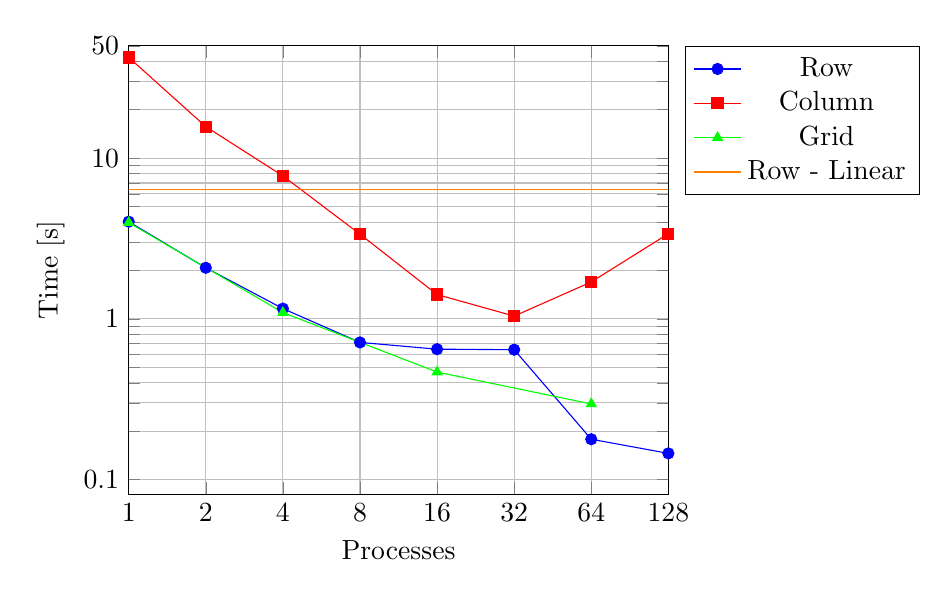
\begin{tikzpicture}
    \begin{axis}[
        xlabel={Processes},
        ylabel={Time [s]},
        legend pos=outer north east, % Adjust the legend position
        grid=both, % Display grid lines
        xmode=log, % Set x-axis to logarithmic scale
        ymode=log,
        xmin=1, xmax=128, % Set x-axis limits
        ymin=0, ymax=50, % Set y-axis limits
        xtick={1,2,4,8,16,32,64,128}, % Specify the x-axis tick values
        ytick={0.1,0.2,0.3,0.4,0.5,0.6,0.7,0.8,0.9,1,2,3,4,5,6,7,8,9,10,20,30,40,50}, % Specify the y-axis tick values you want to label
        yticklabels={0.1,\phantom{a},\phantom{a},\phantom{a},\phantom{a},\phantom{a},\phantom{a},\phantom{a},\phantom{a},1,\phantom{a},\phantom{a},\phantom{a},\phantom{a},\phantom{a},\phantom{a},\phantom{a},\phantom{a},10,\phantom{a},\phantom{a},\phantom{a},50}, % Specify the labels for the y-axis tick values you want to label
        xticklabels={1,2,4,8,16,32,64,128}, % Specify the labels for the tick values
      ]
      
      % Line 1
      \addplot[blue, mark=*, mark options={blue}] coordinates {
        (1,4.02475)
        (2,2.07932)
        (4,1.15842)
        (8,0.713717)
        (16,0.647709)
        (32,0.64301)
        (64,0.178271)
        (128,0.145551)
      };
      \addlegendentry{Row}
      
      % Line 2
      \addplot[red, mark=square*, mark options={red}] coordinates {
              (1,42.3427) 
              (2,15.7043)
              (4,7.75336) 
              (8,3.36393)
              (16,1.41673)
              (32,1.04024)
              (64,1.69703)
              (128,3.3874)
      };
      \addlegendentry{Column}
      
      % Line 3
      \addplot[green, mark=triangle*, mark options={green}] coordinates {
              (1,3.97187)
              (4,1.09431)
              (16,0.466605)
              (64,0.295661)
      };
      \addlegendentry{Grid}
      \addplot[orange] coordinates {
        (1,6.34598)
        (128,6.34598)
      };
      \addlegendentry{Row - Linear}
      
      
    \end{axis}
  \end{tikzpicture}
  \caption{Total time - scale 15}
\end{figure}
\end{frame}
\begin{frame}
\frametitle{Results of communication times}
\begin{figure}
  \centering
  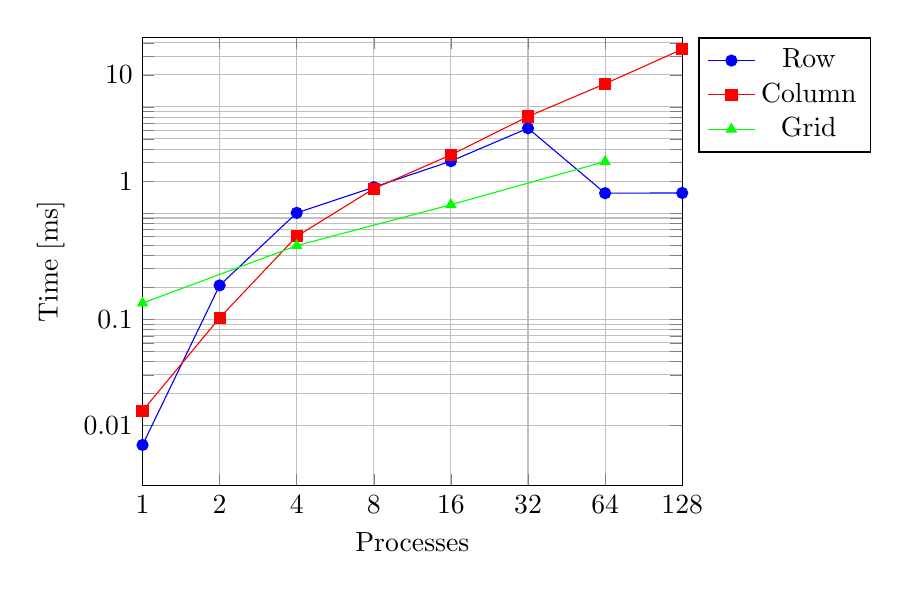
\begin{tikzpicture}
    \begin{axis}[
        xlabel={Processes},
        ylabel={Time [ms]},
        legend pos=outer north east, % Adjust the legend position
        grid=both, % Display grid lines
        xmode=log, % Set x-axis to logarithmic scale
        ymode=log,
        xmin=1, xmax=128, % Set x-axis limits
        ymin=0, ymax=45, % Set y-axis limits
        xtick={1,2,4,8,16,32,64,128}, % Specify the x-axis tick values
        ytick={0.01,0.02,0.03,0.04,0.05,0.06,0.07,0.08,0.09,0.1,0.2,0.3,0.4,0.5,0.6,0.7,0.8,0.9,1,2,3,4,5,6,7,8,9,10,20,30,40},% Specify the x-axis tick values
        yticklabels={0.01,\phantom{a},\phantom{a},\phantom{a},\phantom{a},\phantom{a},\phantom{a},\phantom{a},\phantom{a},0.1,,\phantom{a},\phantom{a},\phantom{a},\phantom{a},\phantom{a},\phantom{a},\phantom{a},\phantom{a},1,\phantom{a},\phantom{a},\phantom{a},\phantom{a},\phantom{a},\phantom{a},\phantom{a},\phantom{a},10,\phantom{a},\phantom{a},40}, % Specify the x-axis tick values
        xticklabels={1,2,4,8,16,32,64,128}, % Specify the labels for the tick values
      ]
      
      % Line 1
      \addplot[blue, mark=*, mark options={blue}] coordinates {
              (1,6.57308e-03)
              (2,0.208763)
              (4,1.0055)
              (8,1.75302)
              (16,3.08256)
              (32,6.28933)
              (64,1.53909)
              (128,1.54738)
      };
      \addlegendentry{Row}
      
      % Line 2
      \addplot[red, mark=square*, mark options={red}] coordinates {
              (1,1.37777e-02)
              (2,0.103341)
              (4,0.604595)
              (8,1.69822)
              (16,3.53032)
              (32,8.10178)
              (64,16.4949)
              (128,34.8204)
      };
      \addlegendentry{Column}
      
      % Line 3
      \addplot[green, mark=triangle*, mark options={green}] coordinates {
              (1,0.14213)
              (4,0.49376)
              (16,1.19948)
              (64,3.05434)
      };
      \addlegendentry{Grid}
      
      
    \end{axis}
  \end{tikzpicture}
  \caption{Total communication time - scale 15}
\end{figure}
\end{frame}

\begin{frame}
\frametitle{Row Based - with vs without \texttt{\#pragma omp paralell for}}
\begin{figure}
  \centering
  \begin{tikzpicture}
    \begin{axis}[
        width=0.8\textwidth, % Adjust the width of the plot
        height=0.7\textheight, % Adjust the height of the plot
        xlabel={Processes},
        ylabel={Time [s]},
        legend pos=outer north east, % Adjust the legend position
        grid=both, % Display grid lines
        xmode=log, % Set x-axis to logarithmic scale
        ymode=log,
        xmin=1, xmax=128, % Set x-axis limits
        ymin=0, ymax=10, % Set y-axis limits
        xtick={1,2,4,8,16,32,64,128}, % Specify the x-axis tick values
        ytick={0.1,0.2,0.3,0.4,0.5,0.6,0.7,0.8,0.9,1,2,3,4,5,6,7,8,9,10,20,30,40,50}, % Specify the y-axis tick values you want to label
        yticklabels={0.1,\phantom{a},\phantom{a},\phantom{a},\phantom{a},\phantom{a},\phantom{a},\phantom{a},\phantom{a},1,\phantom{a},\phantom{a},\phantom{a},\phantom{a},\phantom{a},\phantom{a},\phantom{a},\phantom{a},10,\phantom{a},\phantom{a},\phantom{a},50}, % Specify the labels for the y-axis tick values you want to label
        xticklabels={1,2,4,8,16,32,64,128}, % Specify the labels for the tick values
      ]
      
      % Line 1
      \addplot[blue, mark=*, mark options={blue}] coordinates {
        (1,0.525434)
        (2,0.451033)
        (4,0.422788)
        (8,0.489844)
        (16,0.710966)
        (32,0.86922)
        (64,0.487559)
        (128,0.509738)
      };
      \addlegendentry{with}
      
      % Line 2
      \addplot[red, mark=square*, mark options={red}] coordinates {
        (1,4.02475)
        (2,2.07932)
        (4,1.15842)
        (8,0.713717)
        (16,0.647709)
        (32,0.64301)
        (64,0.178271)
        (128,0.145551)
      };
      \addlegendentry{without}
    \end{axis}
  \end{tikzpicture}
  \caption{Total time - scale 15}
\end{figure}
\end{frame}
\begin{frame}
\frametitle{Column Based - with vs without \texttt{\#pragma omp paralell for}}
\begin{figure}
  \centering
  \begin{tikzpicture}
    \begin{axis}[
        width=0.8\textwidth, % Adjust the width of the plot
        height=0.7\textheight, % Adjust the height of the plot
        xlabel={Processes},
        ylabel={Time [s]},
        legend pos=outer north east, % Adjust the legend position
        grid=both, % Display grid lines
        xmode=log, % Set x-axis to logarithmic scale
        ymode=log,
        xmin=1, xmax=128, % Set x-axis limits
        ymin=0, ymax=50, % Set y-axis limits
        xtick={1,2,4,8,16,32,64,128}, % Specify the x-axis tick values
        ytick={0.1,0.2,0.3,0.4,0.5,0.6,0.7,0.8,0.9,1,2,3,4,5,6,7,8,9,10,20,30,40,50}, % Specify the y-axis tick values you want to label
        yticklabels={0.1,\phantom{a},\phantom{a},\phantom{a},\phantom{a},\phantom{a},\phantom{a},\phantom{a},\phantom{a},1,\phantom{a},\phantom{a},\phantom{a},\phantom{a},\phantom{a},\phantom{a},\phantom{a},\phantom{a},10,\phantom{a},\phantom{a},\phantom{a},50}, % Specify the labels for the y-axis tick values you want to label
        xticklabels={1,2,4,8,16,32,64,128}, % Specify the labels for the tick values
      ]
      
      % Line 1
      \addplot[blue, mark=*, mark options={blue}] coordinates {
        (1,2.98272)
        (2,2.57032)
        (4,2.45381)
        (8,1.92104)
        (16,1.1088)
        (32,1.65221)
        (64,2.62607)
        (128,5.04439)
      };
      \addlegendentry{with}
      
      % Line 2
      \addplot[red, mark=square*, mark options={red}] coordinates {
              (1,42.3427) 
              (2,15.7043)
              (4,7.75336) 
              (8,3.36393)
              (16,1.41673)
              (32,1.04024)
              (64,1.69703)
              (128,3.3874)
      };
      \addlegendentry{without}
    \end{axis}
  \end{tikzpicture}
  \caption{Total time - scale 15}
\end{figure}
\end{frame}
\begin{frame}
\frametitle{Grid Based - with vs without \texttt{\#pragma omp paralell for}}
\begin{figure}
  \centering
  \begin{tikzpicture}
    \begin{axis}[
        width=0.8\textwidth, % Adjust the width of the plot
        height=0.7\textheight, % Adjust the height of the plot
        xlabel={Processes},
        ylabel={Time [s]},
        legend pos=outer north east, % Adjust the legend position
        grid=both, % Display grid lines
        xmode=log, % Set x-axis to logarithmic scale
        ymode=log,
        xmin=1, xmax=64, % Set x-axis limits
        ymin=0, ymax=10, % Set y-axis limits
        xtick={1,4,16,64}, % Specify the x-axis tick values
        ytick={0.1,0.2,0.3,0.4,0.5,0.6,0.7,0.8,0.9,1,2,3,4,5,6,7,8,9,10,20,30,40,50}, % Specify the y-axis tick values you want to label
        yticklabels={0.1,\phantom{a},\phantom{a},\phantom{a},\phantom{a},\phantom{a},\phantom{a},\phantom{a},\phantom{a},1,\phantom{a},\phantom{a},\phantom{a},\phantom{a},\phantom{a},\phantom{a},\phantom{a},\phantom{a},10,\phantom{a},\phantom{a},\phantom{a},50}, % Specify the labels for the y-axis tick values you want to label
        xticklabels={1,4,16,64}, % Specify the labels for the tick values
      ]
      
      % Line 1
      \addplot[blue, mark=*, mark options={blue}] coordinates {
              (1,0.532767)
              (4,0.433744)
              (16,0.704055)
              (64,0.656142)
      };
      \addlegendentry{with}
      
      % Line 2
      \addplot[red, mark=square*, mark options={red}] coordinates {
              (1,3.97187)
              (4,1.09431)
              (16,0.466605)
              (64,0.295661)
      };
      \addlegendentry{without}
    \end{axis}
  \end{tikzpicture}
  \caption{Total time - scale 15}
\end{figure}
\end{frame}
\end{document}

